%Emitter
\section{\acl{AODCS}}
\label{emDDadcs}
To be able to perform its mission the attitude and orbit of the emitter satellite need to be accurately determined and controlled. The \ac{AODCS} of the satellite can be split up into a number of components, which are all described separately in this section. Section \ref{ss:emDDads} covers the attitude determination, section \ref{ss:emDDacs} describes the attitude control, the orbit determination is threaded in section \ref{ss:emDDods} and section \ref{ss:emDDocs} concerns the orbit control. Furthermore section \ref{ss:emDDpoint} is about the pointing mechanism for the emitter. Section \ref{ss:emDDoverview} gives an overview of the mass, costs and power for the complete \ac{AODCS} and pointing mechanism.

%%%%%%%%%%%%%%%%%%%%%%%%%%%%%%%%%%%%%%%%%%%%%%%%%%%%%%%%%%%%%%%%%%%%%
\subsection{Attitude Determination}
\label{ss:emDDads}
In the Midterm Report \cite{midterm} a combination of sun sensors, for the day (Sunlit) phase, and a star tracker, for the night (eclipse) phase, was chosen for the attitude determination of the satellites. A total of five sun sensors is used, one on the top of the satellite and one on each of the side walls. Since the satellite is nadir pointing no sun sensor on the bottom of the satellite is required. The star tracker is located on the top of the satellite, so it will always be pointed towards space.

The sun sensors used are the \ac{CoSS} from TNO \cite{tnoweb}, the left image in figure \ref{fig:sunstar} on page \pageref{fig:sunstar} shows the instrument. The mass of the instrument is 24 grams and it has a volume of 30 x 30 x 14.5 $mm^3$. It has a full cone view angle of 160${}^\circ$ and an accuracy of about 3 arcsec. The cost of one of these sun sensors is 11000 EUR, including all documentation and cables. Since the sensors are passive no external power is needed. It has to be noted for the processing of the data that analogue sun sensors in \ac{LEO} are sensitive to the influence of Earth albedo.

There are currently still few star trackers available for micro-satellites because of their complexity and consequential size. Aeroastro has developed a star tracker with a mass of 375 grams and dimensions of 60 x 76.2 x 76.2 $mm^3$ (excluding a baffle) shown in the right image in figure \ref{fig:sunstar} on page \pageref{fig:sunstar}. The instrument has a field of view of 24 x 30 degrees. It uses less than 2 Watts (1 Watt nominal) of power. The attitude determination accuracy is about 90 arcsec. Up to 9 stars can be tracked at a time. \ac{ISIS} \cite{cubesatshop} is working on a similar star tracker. Their dimensions are 50 x 50 x 100 $mm^3$. The instrument is planned to be ready for flight mid 2011 and will cost about 75000 EUR. 

\begin{figure} [h]
\centering
\begin{tabular}{c c}
%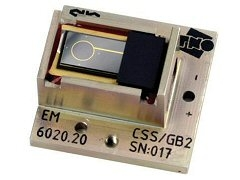
\includegraphics[width = 0.4\textwidth]{chapters/img/CoSS.jpg} & 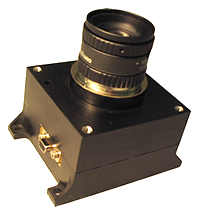
\includegraphics[width = 0.4\textwidth]{chapters/img/MSTracker.png}
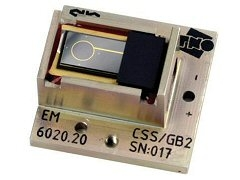
\includegraphics[width = 0.4\textwidth, bb=0 0 240px 180px]{chapters/img/CoSS.jpg} & 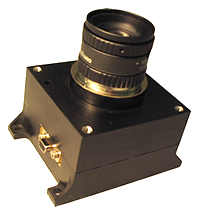
\includegraphics[width = 0.4\textwidth, bb=0 0 219px 215px]{chapters/img/MSTracker.png}
\end{tabular}
\caption[Sun sensor and star tracker]{The TNO Cosine Sun Sensor \cite{tnoweb} and the Aeroastro Miniature Star Tracker \cite{aeromst}}
\label{fig:sunstar}
\end{figure}

%%%%%%%%%%%%%%%%%%%%%%%%%%%%%%%%%%%%%%%%%%%%%%%%%%%%%%%%%%%%%%%%%%%%%
\subsection{Attitude Control}
\label{ss:emDDacs}
The attitude control of the satellites in the Laser Swarm is done by reaction wheels for manoeuvring and magnetic torquers for desaturation (spinning down) of the wheels. 

The size of the reaction wheels is such that the system is able to counter all disturbance torques that work on the satellite. The main disturbance torques are caused by the Earth's gravity gradient $T_g$(equation \ref{distgg}), Solar radiation $T_{sp}$ (equation \ref{distsr}), the Earth magnetic field $T_m$ (equation \ref{distmf}) and aerodynamics $T_a$ (equation \ref{distae}) \cite{larson}.

\begin{eqnarray}
T_g \,&=& \frac{3\mu}{2R^3} \left|I_z - I_y \right| \sin{2\theta} \label{distgg} \\
T_{sp} &=& \frac{F_s}{c}A_s\left(1+q\right)\cos{i}\left(c_{ps}-cg\right) \label{distsr} \\
T_m \,&=& DB \label{distmf} \label{distmf} \\
T_a \,&=& \dfrac{1}{2}\rho C_dAV^2 \left(c_{pa} -cg\right) \label{distae}
\end{eqnarray}
where $\mu$ is the Earth's gravitational constant 398600.4418 $km^3/s^2$, $R$ is the radius of the orbit, $I$ is the satellite inertia tensor, $\theta$ is the deviation from nadir, $F_s$ is the Solar constant 1367 $W/m^2$, $c$ is the speed of light 299792458 $m/s$, $q$ is the reflectance factor (between 0-1, typically 0.6), $i$ is the angle of incidence of the Sun, $c_{ps}$ is the center of solar pressure, $cg$ is the center of gravity, $D$ is the residual dipole of the satellite in $A\cdot m^2$, $B$ can be approximated as $2M/R^3$ in Tesla, where $M$ is the magnetic moment of the Earth 7.96 $T\cdot 10^{15} m^3$, $\rho$ is the local density in $kg/m^3$, $C_d$ is the drag coefficient of the satellite, $A$ is the surface area in $m^2$, $V$ is the satellite velocity and $c_{pa}$ is the center of aerodynamic pressure.

Filling out equations \ref{distgg} to \ref{distae} with realistic numbers for the emitter satellite results in

\begin{eqnarray*}
T_g \,=& \frac{3\cdot 398600.4\cdot 10^9}{2\cdot 6878000^3} \left| 6.542 - 2.407 \right| \sin{\left(2\cdot 1^\circ \right)} &= 2.652\cdot 10^{-7}\,Nm\\
T_{sp} =& \frac{1367}{3\cdot 10^8}1.58\left(1+0.6\right)\cos{0^\circ}\left(0.2\right) &= 2.304 \cdot 10^{-6}\,Nm\\
T_m \,=& 4.893\cdot 10^{-5} \cdot 1  &= 4.893\cdot 10^{-5}\,Nm\\
T_a \,=& \dfrac{1}{2} 1.80 \cdot 10^{-12}\cdot 2.2\cdot 1.58 \cdot 7613^2 \left(0.2\right) &= 3.626 \cdot 10^{-5}\,Nm
\end{eqnarray*}

Using the values and from SMAD \cite{larson}. The moments or inertia of the satellite are $I_x = 2.407\,kgm^2$,  $I_y = 5.582\,kgm^2$ and $I_z = 6.542\,kgm^2$ derived from  from the model. The maximum total disturbance torque expected on the satellite is the sum of all the above torques, i.e. $8.776 \cdot 10^{-5}\,Nm$. For redundancy a margin of 2 is standard, so the torque the reaction wheels have to be able to produce is $1.755\cdot 10^{-4}\,Nm$.

The motors chosen for the reaction wheels are the Faulhauber 2209 Brushless DC-micromotors. The mass of the motor is 8.5 grams, the dimensions 22 x 22 x 17,5 $mm^3$ and the maximal rotation speed is 10000 rpm \cite{faulhaber}. They cost 176 EUR a piece. The maximum angular acceleration $\dot{\omega}_{max}$ they can perform is $1.03\cdot 10^3\,rad/s^2$. 

Figure \ref{fig:wheel} on page \pageref{fig:wheel} shows the general layout of a general reaction wheel suitable for the motor. Wheel basically consists of two integrated parts, a top ring and a side skirt. The top ring has a standard thickness of 1, the height $h$ and width $b$ of the skirt can be adapted to fit the requirements. 

\begin{figure}
\centering
%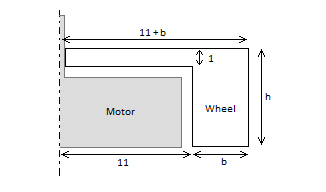
\includegraphics[width=0.3\textwidth]{chapters/img/reactionwheel.png}
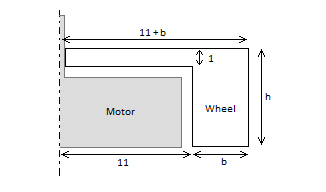
\includegraphics[width=0.3\textwidth, bb=0 0 216px 190px]{chapters/img/reactionwheel.png}
\caption[Basic reaction wheel]{The general layout of a one of the reaction wheels. The motor is depicted in grey, the wheel in white.}
\label{fig:wheel}
\end{figure}

The torque a reaction wheel can produce is determined by

\begin{equation}
T_w = I_w \dot{\omega}_w
\label{wheeltorque}
\end{equation}

where $I_w$ is the inertia tensor of the wheel and $\dot{\omega}_w$ the angular acceleration. The inertia of the wheel depends on the dimensions.  The basic build-up of the wheels is a disk with a skirt around the motor giving the mass at a distance from the rotation axis as shown in figure \ref{fig:wheel} on page \pageref{fig:wheel}. The thickness $b$ of the skirt is 8 mm for the yaw wheel and 5 mm for the other two, since the yaw wheel is also used for the instrument pointing increasing the torque requirements. Since the wheel is spinning it is required that the material of the wheel does not produce a magnetic field while rotating, therefore aluminium is chosen for the material. It has a density of $2850 kg/m^3$. The mass of the wheel is 

\begin{equation}
m_w = m_{wd} + m_{ws} = \rho \pi \left(11\cdot 10^{-3}+b\right)^2 1\cdot 10^{-3} + \rho \pi \left(\left(11\cdot 10^{-3}+h\right)^2 - \left(11\cdot 10^{-3}\right)^2\right)\left(b-1\cdot 10^{-3}\right)^2
\end{equation}

where $m_{wd}$ is the mass of the disk, $m_{ws}$ is the mass of the skirt, $b$ is the thickness of the skirt and $h$ is the height. The moment of inertia of the wheel can then be calculated as

\begin{equation}
I_w =  m_{wd} \cdot \left(\frac{11\cdot 10^{-3}+b}{2}\right)^2  + m_{ws} \cdot \left(11\cdot 10^{-3}+\frac{b}{2}\right)^2
\end{equation}

By taking an angular acceleration of 100 rad/s and taking a wheel height $h$ of 1 cm the wheel skirt thickness $b$ of 36 mm is required. The mass is 212 grams per wheel. The inertia of the motor is not considered.

The magnetic torquer chosen for the emitter is the MT2-1, it can deliver a dipole moment of 2.0 $Am^2$, a mass of 0.2 kg a length of 157.5 mm and a diameter of 15 mm \cite{zarm}. They use a linear power of 0.5 Watt. Three are needed in orthogonal planes to be able to desaturate all wheels.

%%%%%%%%%%%%%%%%%%%%%%%%%%%%%%%%%%%%%%%%%%%%%%%%%%%%%%%%%%%%%%%%%%%%%
\subsection{Orbit Determination}
\label{ss:emDDods}
The orbit determination will be done using the navigation subsystem, which is described in section \ref{NaviEmitter}.

%%%%%%%%%%%%%%%%%%%%%%%%%%%%%%%%%%%%%%%%%%%%%%%%%%%%%%%%%%%%%%%%%%%%%
\subsection{Orbit Control}
\label{ss:emDDocs}
In section \ref{} the $\Delta V$ required for the emitter satellite is 221 m/s. Because the main manoeuvre of the satellite is the boost to a higher orbit a bipropellent thruster, an EADS' 10 N Bipropellant Thruster Model S10 - 23 is chosen \cite{10Nthruster}. This kind of thruster has already flown on over 90 satellites. The specific impulse $I_{sp}$ delivered by the thruster is 291s. The mass of the dual seat valve model is 650 grams, the general dimensions are 90.3 x 37.4 x 178.5 $mm^3$. The throat diameter is 2.85 mm and the diameter of the exit is 35 mm. By filling out the equation for the fuel mass over dry mass ratio

\begin{equation}
\frac{m_p}{m_0} = 1 - e^{-\Delta V/(I_{sp}g)}
\label{fuelratio}
\end{equation}

the amount of fuel needed is 7.5\% of the dry mass of the satellite needs to be fuel. For the 50.4 kg satellite the fuel mass is therefore 3.8 kg. The thruster works on a 1:1.5 mixture dinitrogen tetroxide $N_2O_4$ and monomethylhydrazine $MMH$. This leads to fuel masses of 1.5 kg of $N_2O_2$ and 2.3 kg of $MMH$, with the typical bulk densities noted in \cite{larson} this leads to volumes of 1.32 and 2.88 litres respectively.

%%%%%%%%%%%%%%%%%%%%%%%%%%%%%%%%%%%%%%%%%%%%%%%%%%%%%%%%%%%%%%%%%%%%%
\subsection{Pointing Mechanism}
\label{ss:emDDpoint}
Since the \acs{laser} and satellite will both always be nadir pointing no additional pointing mechanism for the \acs{laser} is needed. The receiver on the emitter satellite also does not require a pointing mechanism since the ground target will always be on same horizontal point under the satellite. Because the satellite is moving in its orbit during the travel time of the signal the receiver instrument possibly could have to look at a small angle slightly behind the satellite to receive a reflected signal from the ground. The pulse travels two times 500 $km$, from orbit to ground and vice versa, in 3.34 $ms$. In that time the satellite covers 25.4 meters. Therefore the instrument needs to point back 0.003 degrees to always have the optimal signal in the middle of the receiver. Since the pointing accuracy required is only 0.1 degree there is no need for a back looking receiver instrument.

%%%%%%%%%%%%%%%%%%%%%%%%%%%%%%%%%%%%%%%%%%%%%%%%%%%%%%%%%%%%%%%%%%%%%
\subsection{Overview}
\label{ss:emDDoverview}
In table \ref{tab:adcspointbudgetemitter} on page \pageref{tab:adcspointbudgetemitter} an overview is given of all masses, costs and power requirements of the \ac{ADCS}, \ac{ODCS} and the pointing mechanism. Since the basic structure of the satellite will not be able to carry all loads of the subsystems some extra mass is added for supporting the components ensuring that correct pointing of sensors, instruments and actuators.

\begin{table}[h]
\begin{tabular}{l | c | c c | c c | c }
Subsystem component    & Number & Mass & Cost & Total mass & Total cost & Power (max)\\ 
                       &   & [g] & [EUR]& [g]  &[EUR] & [W]         \\ \hline \hline
Sun sensors            & 5 & 24  & 11000& 120   & 55000&  0 (0)      \\
Star trackers          & 1 & 375 & 75000& 375  & 75000&  1 (2)      \\ \hline
Reaction wheel motors  & 3 & 8.5 & 176  & 25.5 & 528  &  0.15 (1.5) \\
Reaction wheel disk    & 3 & 36  & 10*  & 108   & 30*  &  0 (0)      \\
Magneto torquers       & 3 & 200 & 3000 & 600  & 9000 &  1.5 (3)      \\ \hline
Thruster			   & 1 & 650 & 400k & 650  & 400k &  1 (2)			\\
Fuel tanks, pumps	   & 2 & 500 & 250* & 1000 & 500* & 0 (0)          \\ \hline
Support structures     & - &  -  & -	& 770  & 300*     & 0 (0)			\\ \hline
Total & & &                             & 3650 & 540k & 3.65 (4.4 rms) \\
&&&&& 310k FY00\$ &
\end{tabular}
\caption[Mass, cost and power budget of AODCS and pointing mechanism emitter]{Dry mass, cost and power budget of different parts of the \ac{ADCS} and pointing mechanism. Starred prices are estimations based on material and machining cost.}
\label{tab:adcspointbudgetemitter}
\end{table}